 \documentclass{include/protokollclass}
% Main File - Based on protokollclass.cls
% Comments are mostly in English (and some in German, concerning the Praktikum)
% ------------------------------------------------------------------------------
% Further files in folder:
%  - include/cmds.tex (for macros and additional commands)
%  - include/kitlogo.pdf (for titlepage)
%  - lit.bib (bibtex bibliography database)
%  - include/titlepage.tex (for layout of titelpage)
% ------------------------------------------------------------------------------
% Useful Supplied Packages:
% amsmath, amssymb, mathtools, bbm, upgreek, nicefrac,
% siunitx, varioref, booktabs, graphicx, tikz, multicol

\usepackage{rotating}
\usepackage{icomma}
\usepackage{subfig}
\usepackage{pdfpages}
\usepackage[onehalfspacing]{setspace}


%% ---------------------------------------------
%% |    Informationen über dieses Protokoll    |
%% ---------------------------------------------
\newcommand{\praktikum}{P3}                % P1 oder P2
\newcommand{\semester}{WS17/18}            % z.B. "WS14/15" oder "SS15"

\newcommand{\wochentag}{Mi}                % Mo, Di, Mi oder Do
\newcommand{\gruppennr}{144}                % Zweistellige Gruppennummer

\newcommand{\nachnamea}{Friedrich}             % Nachname des ersten Praktikanten
\newcommand{\vornamea}{Tabea}               % Vorname des ersten Praktikanten
\newcommand{\nachnameb}{Stockmeier}              % Nachname des zweiten Praktikanten
\newcommand{\vornameb}{Lea}              % Vorname des zweiten Praktikanten

\newcommand{\emailadressen}{lea.stockmeier@web.de, tabea.friedrich@t-online.de}
% optionale Angabe von Emailadresse(n) für den Kontakt mit dem Betreuer

\newcommand{\versuch}{Gravimetrie} % Name des Versuchs
\newcommand{\versuchsnr}{00}               % bitte die korrekte Nummer dem 
                                           % Arbeitsplatz am Versuchstag 
                                           % entnehmen
\newcommand{\fehlerrechnung}{Ja}         % Ob Fehlerrechnung im Versuch 
                                           % durchgeführt wurde oder nicht

\newcommand{\betreuer}{Betreuer}      % Name des zuständigen Betreuers
\newcommand{\durchgefuehrt}{00.00.17}      % Datum, an dem der Versuch 
                                           % durchgeführt wurde





%% --------------------------------------
%% |    Settings for Word Separation    |
%% --------------------------------------
% Help for separation:
% In German package the following hints are additionally available:
% "- = Additional separation
% "| = Suppress ligation and possible separation (e.g. Schaf"|fell)
% "~ = Hyphenation without separation (e.g. bergauf und "~ab)
% "= = Hyphenation with separation before and after
% "" = Separation without a hyphenation (e.g. und/""oder)

% Describe separation hints here:
\hyphenation
{
    über-nom-me-nen an-ge-ge-be-nen
    %Pro-to-koll-in-stan-zen
    %Ma-na-ge-ment  Netz-werk-ele-men-ten
    %Netz-werk Netz-werk-re-ser-vie-rung
    %Netz-werk-adap-ter Fein-ju-stier-ung
    %Da-ten-strom-spe-zi-fi-ka-tion Pa-ket-rumpf
    %Kon-troll-in-stanz
}





% um die Titelseite per PDF-reader auszufüllen. Vorgefertigte Daten
% können in Datei 'data.tex' modifiziert werden.
%\setboolean{forminput}{true}
% um die Anmerkungen zu den Textfeldern anzeigen zu lassen
%\setboolean{showannotations}{true}
% Erneuern der Seitenzahl in jedem Kapitel
%\setboolean{chapResetPageNumb}{true}
% Einbinden der Kapitelnummer in der Seitenzahl
%\setboolean{chapWiseNumb}{true}
% english or ngerman (new german für neue deutsche Rechtschreibung statt german)
\SelectLanguage{ngerman}

\title{Geophysikalische Geländeübungen \\ SS 2018 \\ Gravimetrie}
\subtitle{Messgebiet A59/1 (Riedheim)}
\author{\\ Svenja Müller \\ mueller-svenja@gmx.net
\\ \\und\\ \\
Lea Stockmeier \\ lea.stockmeier@web.de \\ \\ \\
Betreuer: Vorname1 Nachname1 und Vorname2 Nachname2}
\date{\vfill\vfill\vfill \today}


%% -----------------------
%% |    Main Document    |
%% -----------------------
\begin{document}
    % Titlepage und ToC
    \FrontMatter
    \maketitle


    \begingroup \let\clearpage\relax    % in order to avoid listoffigures and
    \tableofcontents                    % listoftables on new pages
    \listoffigures
%   \listoftables
    \endgroup
    %\cleardoublepage



    % Contents
    \MainMatter
    
    %\emptychapter[1]{Messprotokoll 1}{} % usage: \emptychapter[page displayed 
                                        %        in toc]{name of the chapter}
    %\pseudochapter[3]{Messprotokoll 2}  % usage: \pseudochapter[number of pages 
                                        %        added]{name of the chapter}
    
 %   \pseudochapter[2]{Versuchsbeschreibung}
%    \pseudochapter[4]{Messprotokoll}

    \chapter{Einleitung}
    Die Geoelektrik-Messungen wurde am dritten Messtag, dem 24.05.2018, in Riedheim durchgeführt.

Die Profile waren in den gleichen Messgebieten wie die der anderen Messdurchführungen, um sie vergleichen zu können. Unsere Fragestellungen waren folgende:

Die Kartierung und Tomographie wurde im Messgebiet mit dem Basaltgang durchgeführt. Wir wollen herausfinden, ob der Gang mit diesen Messmethoden lokalisierbar ist und wenn ja wie gut. Die Ergebnisse sollen mit den Ergebnissen der anderen dort angewendeten Methoden verglichen werden.

Die Sondierung wurde entlang des gleichen Profils wie eine Seismik-Messung durchgeführt. Hier ist unsere Fragestellung, ob mit beiden Methoden gleiche Schichtgrenzen gefunden werden können. Dies geht jedoch nur mit der Annahme, dass eine Änderung der seismischen Geschwindigkeiten einhergeht mit einer Änderung der Leitfähigkeit. 






    \chapter{Theoretische Grundlagen}
    \section{Seismische Wellen und Seismik}

Ausgelöst durch zum Beispiel Stöße auf die Erdoberfläche oder Erdbeben, kommt es auf der Erde zur Bewegung der Partikel in der Erdoberfläche. Diese Bewegung breitet sich vom Ursprungsort in alle Richtungen aus. Es wird von seismischen Wellen gesprochen. Abhängig von der Partikelbewegung im Untergrund, gibt es longitudinale und transversale Wellen.

Bei longitudinal polarisierten Wellen schwingen die Partikel parallel zur Ausbreitungsgeschwindigkeit der Welle. Sie werden auch P-Wellen oder Kompressionswellen genannt und haben in homogenen isotropen Medien eine Geschwindigkeit von
\begin{equation}
 \q{v}{P}=\sqrt{\frac{\kappa+\frac{4}{3}\mu}{\rho}} \comma
\end{equation}
wobei $\kappa$ das Volumenkompressionsmodul und $\rho$ die Massendichte ist.

Bei senkrechter Partikelbewegung zur Ausbreitungsgeschwindigkeit ist die Welle transversal polarisiert. Sie Wird auch A-Welle oder Scherwelle genannt und hat in homogenen isotropen Medien eine Ausbreitungsgeschwindigkeit von
\begin{equation}
 \q{v}{S}=\sqrt{\frac{\mu}{\rho}} \fullstop
\end{equation}
Da in Flüssigkeiten $\mu=\e{0}{Pa}$ gilt, können sich in diesen keine Scherwellen ausbreiten.

In der Seismik werden diese Wellen durch zum Beispiel einen Hammer (Hammerschlagseismik) künstlich ausgelöst. In verschiedenen Abständen zur Quelle wird mit  Geophonen die Bodenbewegung gemessen und daraus kann dann auf die Ausbreitungsgeschwindigkeit der Wellen im Untergrund geschlossen werden. Es werden bei der Refraktionsseismik nur die Ersteinsätze betrachtet, es wird also nur die P-Wellengeschwindigkeit $\q{v}{P}$ analysiert, weil diese Größer ist als die S-Wellengeschwindigkeit. Die Ersteinsätze erfolgen also immer durch P-Wellen.

\section{Snelliussches Brechungsgesetz und refraktierte Welle} %oder Strahlenseismik???

Wenn die Wellenlänge der Welle sehr viel kleiner als der Abstand zwischen Quelle und Empfänger ist, können die Wellen als Strahl beschrieben werden. Trifft eine Welle auf eine Schichtgrenze (Grenze zwischen Materialien mit unterschiedlichen Ausbreitungsgeschwindigkeiten), wird sie sowahl reflektiert, als auch in das andere Medium gebrochen. Für die reflektierte Welle gilt das Snelliussche Brechungsgesetz
\begin{equation}
 \frac{\sin(\alpha_1)}{\sin(\alpha_2)}=\frac{v_1}{v_2}\fullstop
\end{equation}
$\alpha_1$ ist dabei der der Einfallswinkel zum Lot hin gemessen und $v_1$ die Geschwindigkeit im Medium, in dem der Strahl auf die Grenzfläche einfällt. $\alpha_2$ ist der Ausfallswinkel zum Lot hin gemessen und $v_2$ die Geschwindigkeit im Medium, in das der Strahl hinein gebrochen wird.

Falls $v_2>v_1$ gilt, ist auch $\alpha_2>\alpha_1$. Sobald $\alpha_2=90^\circ$ gilt, kommt es statt zur Reflektion zur Refraktion. Dies passiert ab dem kritischen Winkel
\begin{equation}
 \sin(\q{\alpha}{k}) =\frac{v_1}{v_2} \fullstop
\end{equation}
Eine Welle, die im kritischen Winkel auf die Grenzfläche auftritt, läuft mit der Geschwindigkeit $v_2$ an der Grenzfläche entlang und strahlt permanent ebenfalls unter dem kritischen Winkel Wellen nach oben ab, die dann wieder die Geschwindigkeit $v_1$ des oberen Mediums haben.
    
    \chapter{Versuchsbeschreibung}
    \section{Messung mit dem Gravimeter}
Die Messung mit den beiden vorhandenen Gravimetern wurde auf dem Profil orthogonal zum Basaltgang durchgeführt. Auf dem gleichen Profil wurden schon Messungen mit allen drei der vorherigen Messverfahren durchgeführt.
Das Messprofil ist in Abb. ??? zu sehen. Da zwei Gravimeter zur Verfügung standen, wurde mit jedem der Messgeräte jeweils jeder zweite Punkt vermessen. Der Messpunkt $G0$ in Abb.??? bezeichnet den Basispunkt der Messung, auf
diesem Punkt wurde mit beiden Gravimetern eine Messung durchgeführt. Bei $G7$ wird das Maximum des Basaltgangs erwartet. Deswegen wurden dort die Messabstände am kleinsten gewählt.

Um die Drift der Messgeräte erfassen und korrigieren zu können wurden jeweils zwei Messungen auf dem selben Profil im Abstand von mehr als einer Stunde durchgeführt. Dies wurde umgesetzt indem man mit den Gravimetern 
einmal das ganze Profil komplett entlang ging und dann mit der zweiten Messung wieder am ersten Messpunkt begonnen hat.

Die Messungen wurden mit Gravimetern des Types LaCoste-Romberg(G) durchgeführt. Da Gravimeter sehr empfindliche Messgeräte sind mussten die Messungen sehr genau und vorsichtig durchgeführt werden. Das Messgerät hat eine 
theoretische Auflösung von 0,01 mGal.

Um einen Messpunkt zu vermessen wurde das Gravimeter zunächst neben den mit zwei Pflöcken markierten Punkt gestellt. Mit Hilfe zweier Libellen wurde es horizontal ausgerichtet. Einer der beiden Pflöcke 
war bis auf Handbreite in den Boden geschlagen und diente zur exakten Messung der Instrumentenhöhe. Diese Höhe sollte bis auf 5\,mm genau bestimmt werden.
Wenn das Gravimeter nicht mehr bewegt wurde, konnte die Arretierung gelöst werden. Solange die Messung durchgeführt wurde, achtete man darauf das sich keine Person dem Messgerät näherte oder sich die Personen in der 
Nähe stark bewegen. Dies war wichtig da es einen sofort sichtbaren Einfluss auf die Messung hatte, wenn sich eine Person genähert hat.
Die Messung wurde immer zu dritt durchgeführt. Eine Person war verantwortlich für einen Sonnenschirm, der über das Messgerät gehalten wurde, eine für das Ablesen der Messwerte 
und eine dritte Person hat das Messprotokoll geführt. Um Die Gezeitenkorrektur berechnen zu können wurde auch direkt die Zeit aufgeschrieben.


\section{Tachymetrie}???
Mit einem elektronischen Tachymeter TC 500 wurde die Lage der Messpunkte, die mit den Gravimetern vermessen wurden, bestimmt. Dazu wurde der Reflektor an dem zu vermessenden Punkt aufgestellt und mit dem Messgerät angepeilt. Mit einem Laser 
wurde die Entfernung gemessen.

\section{Vermessung mit GPS}

Mit einem GPS-Gerät wurden die Pflöcke, mit denen alle Profil-Punkte und sonstigen wichtigen Orte während der Messungen markiert wurden, vermessen. Es wurden die GPS-Koordinaten, die Zeit der Messung und die Art der Lösung des Gleichungssystems gespeichert. Manchmal hatte das Messgerät durch zum Beispiel Bäume keinen Kontakt zu genug Satelliten, sodass die Lage der Punkte nicht so genau wie sonst bestimmt werden konnte.

Bei der Messung selbst musste darauf geachtet werden, dass die Stange an der das Gerät befestigt war, mit einer Punkt-Libelle möglichst genau vertikal ausgerichtet wurde. Außerdem musste ihre Länge notiert werden, um auf die Koordinaten auf Boden-Niveau schließen zu können.
    
    \chapter{Auswertung}
    % Gliederung noch anders!!!???
\section{Laufzeitdiagramm}

% Verweise lieber woanders?
Am Abend nach dem Versuch erhielten wir ausgedruckt alle Seismogramme. Die mit Hammerschlag aufgenommenen direkt gestapelt. Daraus pickten wir die Ersteinsätze. Wie genau gepickt wurde, ist in den Abbildungen ??? bis ??? zu sehen. Die Seismogramme des Profils S11-S12 mit Hammerschlag wurden nicht gepickt, da diese Messung in diesem Protokoll nicht weiter ausgewertet wird. Die zugehörigen Laufzeitdiagramme der Hin- und Rückschüsse befinden sich in Abbildung ???, ??? und ???.

\section{Schichtbestimmung}

\subsection{Profil S31-S32}

Das Laufzeitdiagramm mit eingetragenem Hin- und Rückschuss dieses Profils ist achsensymmetrisch um $x=20$. Daraus lässt sich schließen, dass keine geneigten Schichtgrenzen vorliegen. Aus den 


% Verfahren der Verzögerungszeiten wenn sinnvoll???

    % appendix for more or less interesting calculations
 %   \Appendix
 %   \chapter*{\appendixname} \addcontentsline{toc}{chapter}{\appendixname}
    % to make the appendix appear in ToC without number. \appendixname = 
    % Appendix or Anhang (depending on chosen language)
 %   \section{Messprotokolle}

\begin{figure}[h!]
 \centering
 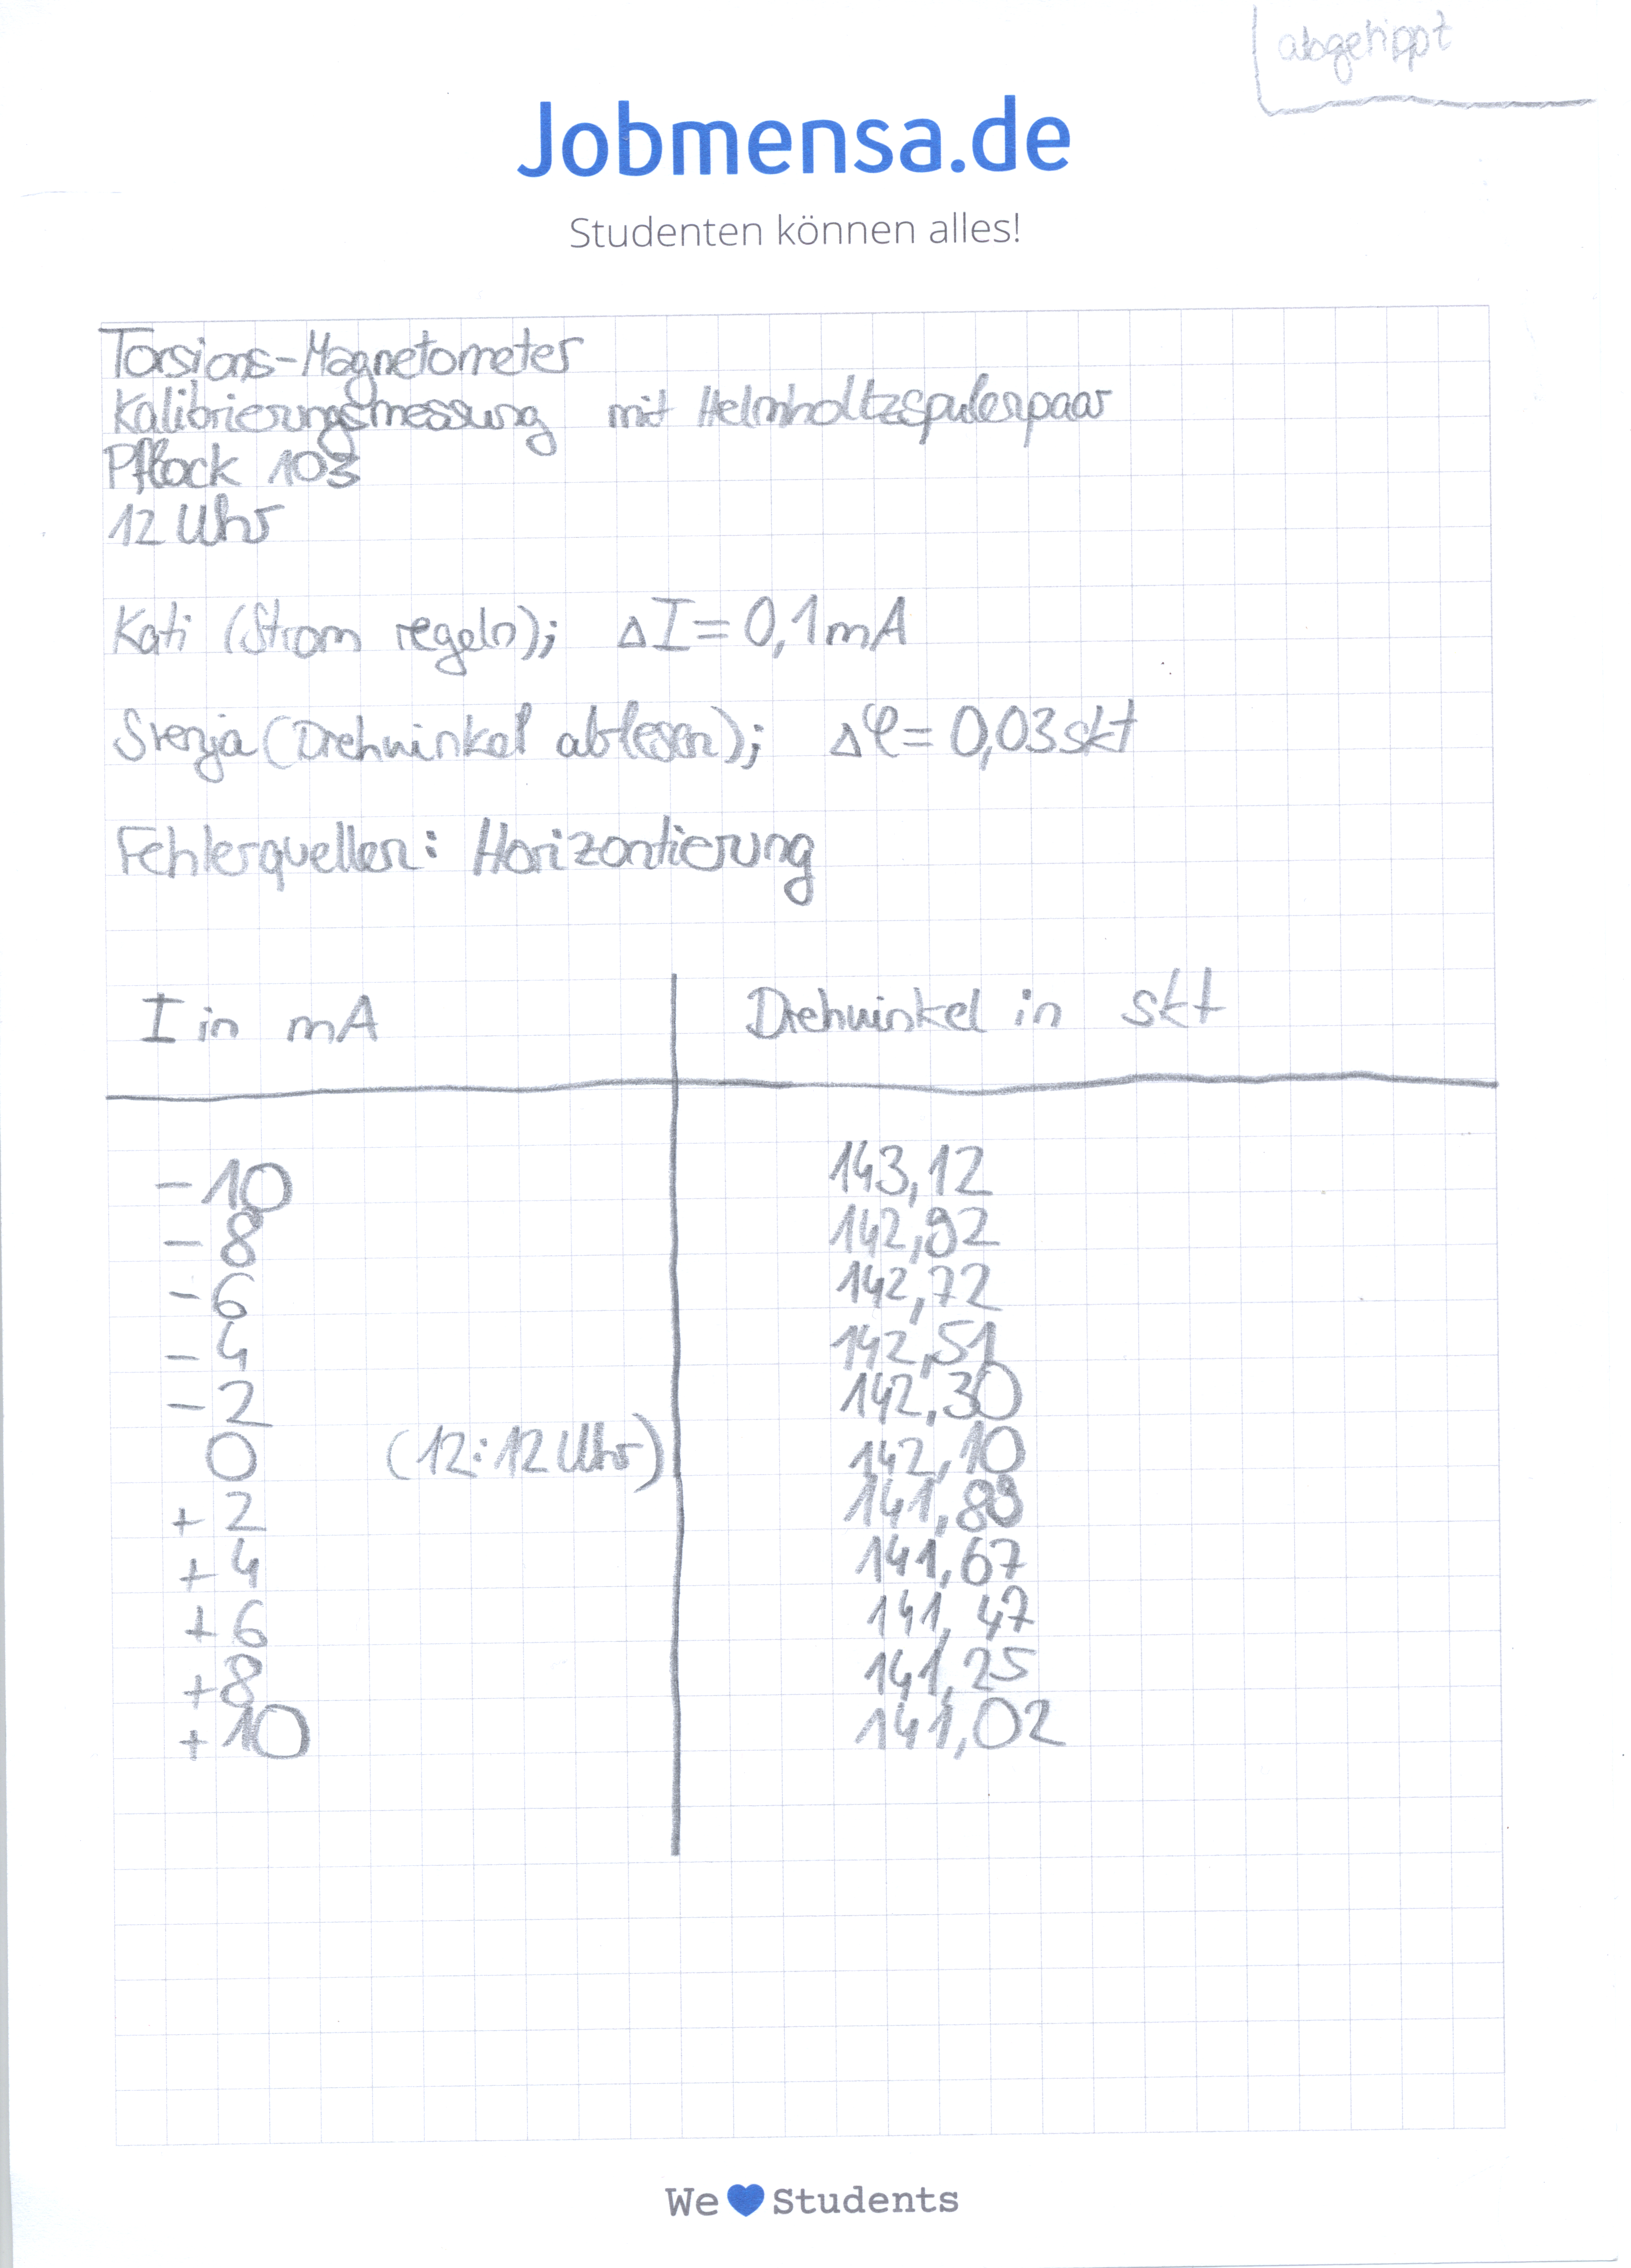
\includegraphics[width=0.8\textwidth]{fig/Messprotokolle/Kalibrierung.png}
 \caption{Messprotokoll zur Kalibrierungsmessung}
 \label{fig:MPKalibrierung}
\end{figure}


% \begin{figure}[h!]
%  \centering
%  \includegraphics[width=\textwidth]{fig/Messprotokolle/}
%  \caption{}
%  \label{fig:}
% \end{figure} %\cleardoublepage



    % Bibliography
    \TheBibliography

    % BIBTEX
    % use if you want citations to appear even if they are not referenced to: 
    % \nocite{*} or maybe \nocite{Kon64,And59} for specific entries
    %\nocite{*}
    \bibliographystyle{babalpha}
    \bibliography{lit.bib}

    % THEBIBLIOGRAPHY
    %\begin{thebibliography}{000}
    %    \bibitem{ident}Entry into Bibliography.
    %\end{thebibliography}
\end{document}
